%Aclaro que no hay consenso en la parte de computo en el borde
%Hacer comparativa entre diferentes perspectivas y definiciones
%Llegar a una definición propia
%Cloud-fog-device podria ser una definición
\section{Arquitectura \textit{Cloud-Fog-Edge Computing}} 
\label{sec:cloud-fog-edge}
La arquitectura cloud-fog-edge representa un enfoque integral para la distribución y gestión eficiente de recursos en entornos distribuidos y heterogéneos. Este paradigma aborda las demandas crecientes de aplicaciones modernas, que requieren procesamiento de datos cercano al punto de generación, así como la capacidad de escalar dinámicamente y aprovechar recursos ubicados de manera remota como lo puede ser una nube.

En este contexto, la arquitectura representada en la Figura \ref{fig:fog} se despliega en tres capas distintas: la nube \textit{(cloud)}, la niebla \textit{(fog)} y el {borde \textit{(edge)}, cada capa tiene características y funcionalidades únicas que se adaptan a diferentes necesidades y restricciones de las aplicaciones y dispositivos.

\begin{figure}
    \centering
    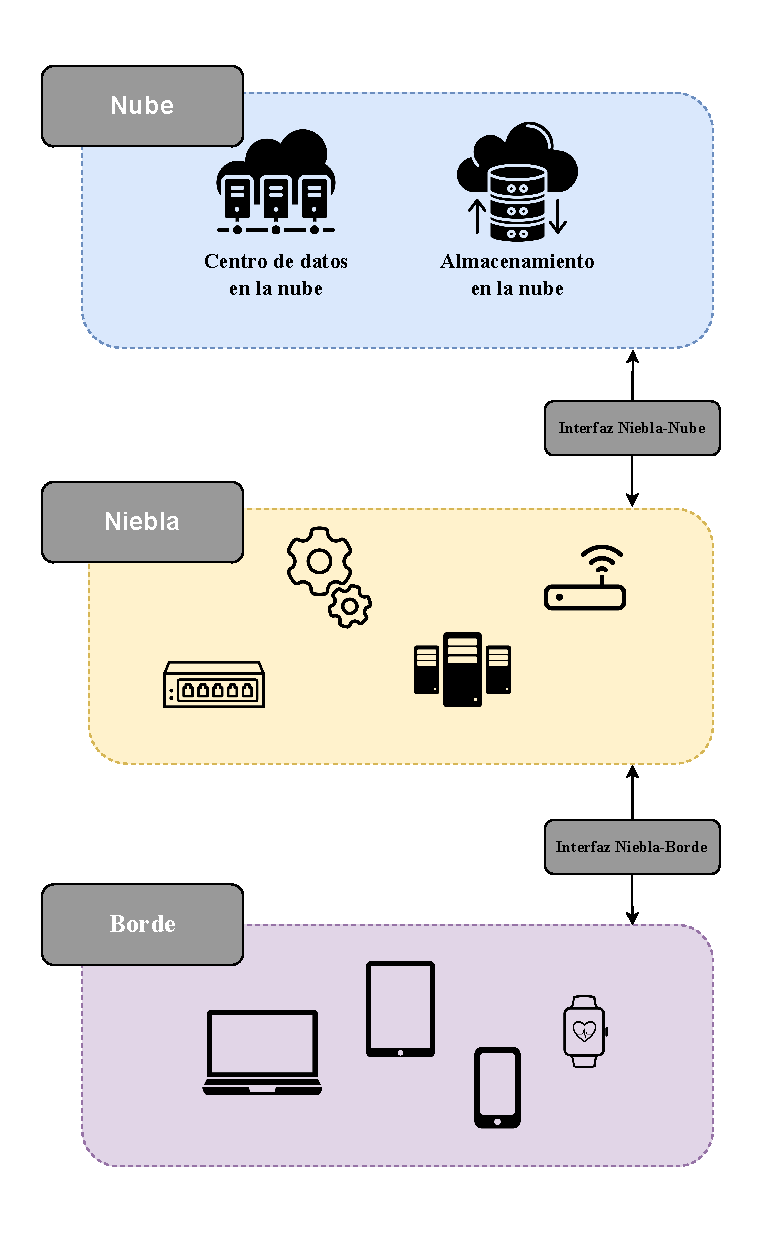
\includegraphics[width=12cm]{Imagenes/Cloud-Fog-Edge/Fog.pdf}
    \caption{Arquitectura de tres capas \textit{cloud-fog-edge}}
    \label{fig:fog}
\end{figure}

La nube es un componente remoto el cual provee servicios de cómputo y/o almacenamiento, usualmente de gran escala, y accesible a través de Internet. Facilita la provisión y el uso de recursos tecnológicos, ofreciendo agilidad, escalabilidad y fácil acceso gracias a una infraestructura flexible y dinámica conectada a través de la red. Además, elimina las limitaciones de infraestructura local y simplifica el acceso a recursos avanzados.

La capa de niebla se ubica más cerca de los dispositivos finales, con el objetivo de actuar como intermediario entre estos y la nube. Ofrece a los dispositivos finales una capacidad de cómputo más grande que la que estos poseen y permite el procesamiento en tiempo real, reduciendo la necesidad de realizar procesamiento de relativamente mayor demanda computacional en servidores de la nube. Al poder ubicarse en la misma red de área local que los dispositivos finales, la capa de niebla permite un alto grado de resiliencia ante fallos de conectividad, pudiendo seguir trabajando con los dispositivos finales por más que se haya perdido conexión con la nube.

La capa de borde está conformada por el conjunto de dispositivos finales, los cuales interactúan directamente con el medio y/o los usuarios, a fin de censar, recolectar y emitir información. Estos dispositivos suelen tener una capacidad de almacenamiento y cómputo reducida, por lo tanto relegan los volúmenes de cómputo más grandes a capas superiores como nube y niebla.





